\documentclass[letterpaper,12pt]{report}
\usepackage[spanish]{babel}
\usepackage[utf8]{inputenc}
\usepackage{graphicx}
\usepackage{amsfonts,amsmath,color,amssymb,float, amsthm,mathrsfs}  
\usepackage[right=3cm,left=2cm,top=2cm,bottom=2cm,headsep=0.7cm,footskip=0.5cm]{geometry}
\usepackage{enumerate}
\usepackage{wrapfig} 
\usepackage[rflt]{floatflt} 
\usepackage{framed}
\usepackage[most]{tcolorbox}
\usepackage{xcolor} 
\colorlet{shadecolor}{green!20}
\setlength\FrameSep{0.5ex}
\usepackage{thmtools}
\usepackage{esint}
\usepackage{cancel}
\usepackage{listings} 
\usepackage{pstricks, caption}
\usepackage[colorlinks]{hyperref}
\usepackage{csquotes}
\usepackage{fullpage}
\usepackage{enumitem}
\usepackage{etoolbox}
\usepackage{tcolorbox}
\usepackage{tikz}
\usetikzlibrary{arrows,babel}


\decimalpoint
\newcommand{\grad}{^\circ}
\newlength{\drop}
\DeclareMathOperator{\sign}{sgn}
\DeclareMathOperator{\Log}{Log}
\providecommand{\norm}[1]{\lVert#1\rVert}

%%%%%%%%%Entornos: Teoremas, Defs,etc%%%%%%%
\theoremstyle{definition}

\newtheorem{defis}{Definiciones}[section]
\newtheorem{corolario}{Corolario}[section] 
\newtheorem{lema}{Lema}[section] 

\newtheorem{protoexample}{Ejemplo}[section]
\newenvironment{ejemplo}
   {\colorlet{shadecolor}{orange!15}\begin{shaded}\begin{protoexample}}
   {\end{protoexample}\end{shaded}}

\newtheorem*{protoproof}{Demostración}
\newenvironment{demo}
   {\colorlet{shadecolor}{blue!10}\begin{shaded}\begin{protoproof}}
   {\end{protoproof}\end{shaded}}

\newenvironment{Rdbleftbar}{%
  \def\FrameCommand{\textcolor{red}{\vrule width0.6pt}\hspace{0.15em}\textcolor{red}{\vrule width0.6pt} \hspace{0.5em}}%
  \MakeFramed {\advance\hsize-\width \FrameRestore}}%
 {\endMakeFramed}

 \newenvironment{Bdbleftbar}{%
  \def\FrameCommand{\vrule width0.6pt\hspace{0.15em}\vrule width0.6pt \hspace{0.5em}}%
  \MakeFramed {\advance\hsize-\width \FrameRestore}}%
 {\endMakeFramed}

\newenvironment{Gdbleftbar}{%
  \def\FrameCommand{\textcolor{green}{\vrule width0.6pt}\hspace{0.15em}\textcolor{green}{\vrule width0.6pt} \hspace{0.5em}}%
  \MakeFramed {\advance\hsize-\width \FrameRestore}}%
 {\endMakeFramed}
 
% With parskip

\usepackage[indent=0.6cm]{parskip}

\declaretheorem[%
name            =Teorema,%
numberwithin=section,
postheadhook    =\vspace*{\parskip} \begin{Rdbleftbar}\vspace*{-5pt},%
prefoothook     =\vspace*{-1pt}\end{Rdbleftbar}%
]{teorema}

\declaretheorem[%
name            =Definición,%
numberwithin=section,
postheadhook    =\vspace*{\parskip}\begin{Bdbleftbar}\vspace*{-5pt},%
prefoothook     =\vspace*{-1pt}\end{Bdbleftbar}%
]{defi}

\declaretheorem[%
name            = Proposición,%
numberwithin=section,
postheadhook    =\vspace*{\parskip}\begin{Gdbleftbar}\vspace*{-5pt},%
prefoothook     =\vspace*{-1pt}\end{Gdbleftbar}%
]{propo}   
%%%%%%%%%%%%%%%%%%%%%%%%%%%%%%%%%%%%%%%%%%%%%%

%%%%%%%%%%%%Fancy Chapters%%%%%%%%%%%%%%%%%
%Options: Sonny, Lenny, Glenn, Conny, Rejne, Bjarne, Bjornstrup
\usepackage[Lenny]{fncychap}
%%%%%%%%%%%%%%%%%%%%%%%%%%%%%%%%%%%%%%%%%%%

%Referencias
\usepackage[backend=biber]{biblatex}
\addbibresource{Referencias.bib}

\begin{document}

\begin{titlepage}
 \drop=0.1\textheight
    \centering
    \vspace*{\baselineskip}
    \rule{\textwidth}{1.6pt}\vspace*{-\baselineskip}\vspace*{2pt}
    \rule{\textwidth}{0.4pt}\\[\baselineskip]
    {\scshape\Huge Física matemática} \\[0.2\baselineskip]
    \rule{\textwidth}{0.4pt}\vspace*{-\baselineskip}\vspace{3.2pt}
    \rule{\textwidth}{1.6pt}\\[\baselineskip]
    {\Large Autor: \par}
{\Large Alejandro Saavedra \par}
\vfill
{\large Diciembre 2022 \par}
{\large v1.0 \par}
\end{titlepage}

\tableofcontents

\chapter{Espacio de funciones}

\section{Definiciones}

\begin{defi}
Denotemos por $\mathcal{C}_0 [a,b]$ al conjunto de funciones complejas continuas de una variable real $t \in [a,b]$.
\end{defi}

Notemos que claramente se cumple:
\begin{shaded}
$$\mbox{si} ~ f,g \in \mathcal{C}_0[a,b] ~\Rightarrow~ f + g \in \mathcal{C}_0 [a,b]$$
\end{shaded}

y 
\begin{shaded}
$$\mbox{si} ~ f \in \mathcal{C}_0[a,b] ~\mbox{y}~ \lambda \in \mathbb{C} ~\Rightarrow~ \lambda f \in  \mathcal{C}_0[a,b].$$ 
\end{shaded}

\begin{defi}
Una función $f: [a,b] \longrightarrow \mathbb{C}$ es \textbf{seccionalmente continua} si $[a,b]$ tiene una partición finita $a = t_0 < t_1 < \cdots < t_n = b$ tal que $f$ es continua y acotada en cada intervalo abierto $]t_i, t_{i+1}[, i = 0, \dots, n-1$.

Denotaremos por $\mathcal{C}[a,b]$ al conjunto de funciones complejas seccionalmente continuas.
\end{defi}

Geométricamente, $f: [a,b] \longrightarrow \mathbb{C}$ es una curva en el plano complejo y la condición de seccionalmente continua se puede apreciar en la figura \ref{fig:FunciónSC}. 

\begin{figure}
    \centering
    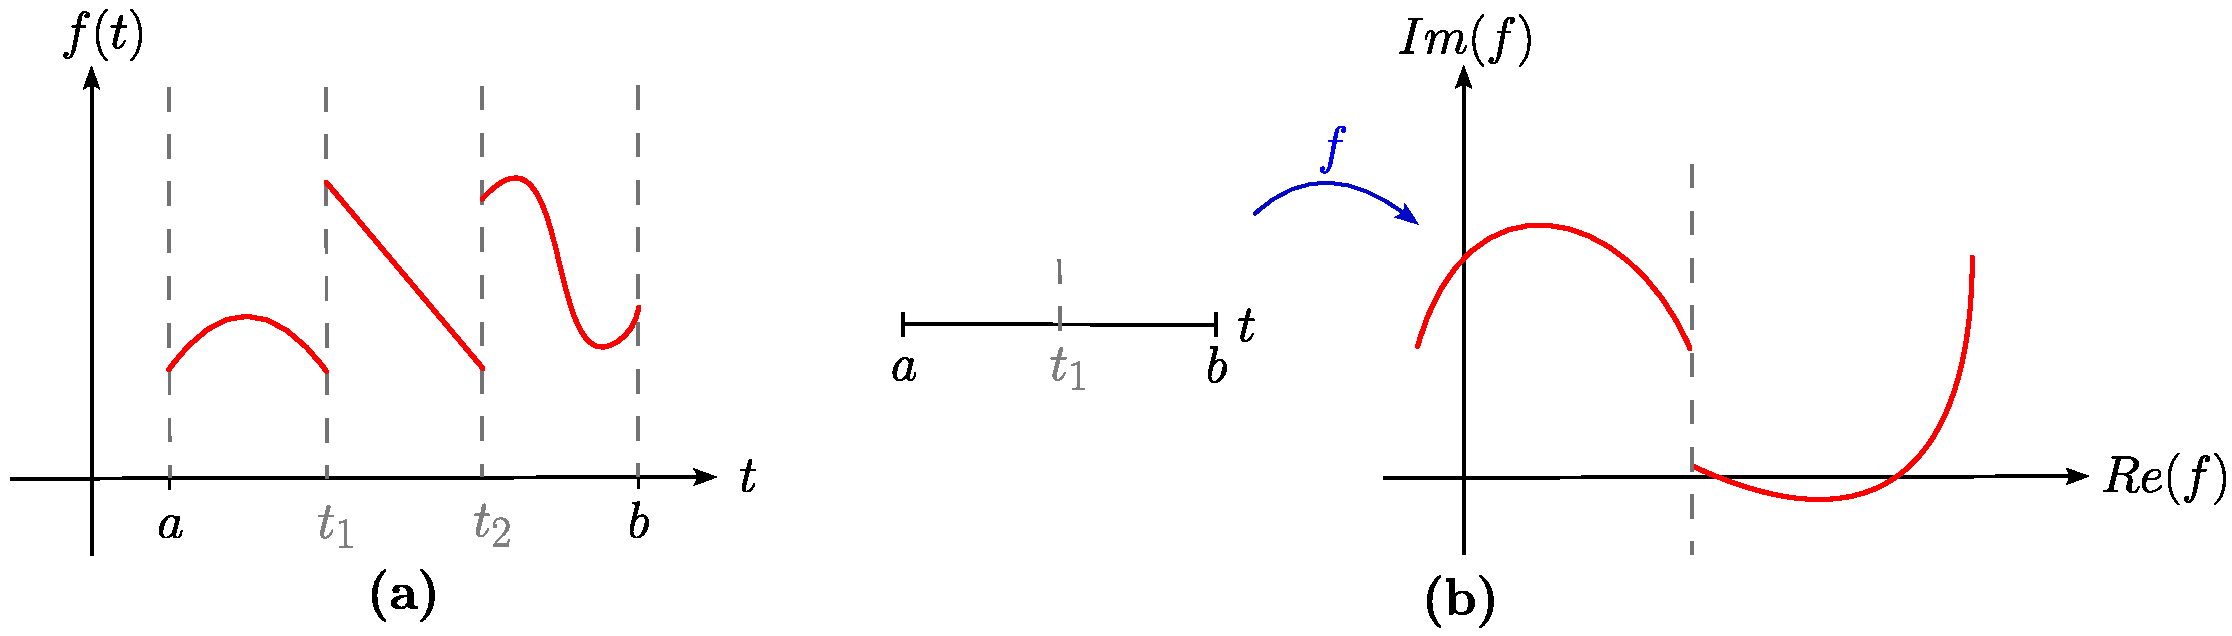
\includegraphics[scale=0.45]{Figuras/FuncionSC.pdf}
    \caption{En (a) una función de la forma $f: [a,b] \rightarrow \mathbb{R}$ y en (b) una función de la forma $f: [a,b] \rightarrow \mathbb{C}$, ambas seccionalmente continuas.}
    \label{fig:FunciónSC}
\end{figure}

Podemos afirmar que los conjuntos $\mathcal{C}_0 [a,b]$ y $\mathcal{C}[a,b]$ forman espacios vectoriales sobre el cuerpo de los complejos. Además, $\mathcal{C}_0 [a,b] \subset \mathcal{C} [a,b].$

\begin{defi}
Consideremos dos funciones $f,g \in \mathcal{C}[a,b]$. Definimos su \textbf{producto escalar} como
$$\boxed{\langle f , g \rangle = \int_a^b f(t) g^*(t) \,dt }$$
\end{defi}

\begin{propo}[Propiedades del producto escalar] \label{ProductoEscalar}
 Sean $f,g,h \in \mathcal{C}[a,b]$ y  $\lambda \in \mathbb{C}$.
 
 \begin{itemize}
     \item $\langle f , g \rangle = \langle g, f \rangle^*$
     \item $\langle f , g + h \rangle = \langle f , g \rangle + \langle f , h \rangle$
     \item $\langle f + g , h \rangle = \langle f , h \rangle + \langle g , h \rangle$
     \item $\langle \lambda f , g \rangle = \lambda \langle f , g \rangle$
     \item $\langle  f , \lambda g \rangle = \lambda^*\langle f , g \rangle$
     \item Si $f \not\equiv 0$, entonces $\langle f , f \rangle > 0$
 \end{itemize}
\end{propo}

\textbf{Observación:} Con respecto a la última propiedad, se tiene que 
$$\langle f , f \rangle = \int_a^b |f(t)|^2 \,dt = 0 ~\mbox{NO IMPLICA}~ f = 0.$$

Por esto se define la relación de equivalencia \footnote{$m(E) = 0$ denota que $E$ es un conjunto de medida cero.}
$$f = g ~ c.t.p ~\Leftrightarrow~ f(t) = g(t), \forall t \in [a,b]-E, \mbox{con}~ m(E) = 0.$$

Esta relación se expresa diciendo que $f = g $ casi en todas partes.

\textbf{Notación:} $f \equiv g ~\Leftrightarrow~ f = g ~c.t.p$

Esencialmente una relación de equivalencia es una relación de igualdad, bajo la cual dos funciones equivalentes se consideran ``iguales". Así, toda función $f = 0 ~c.t.p$, o simplemente $f\equiv 0$, se considera como la función nula.

\begin{defi}
Un espacio vectorial complejo dotado de un producto escalar con las propiedades de la proposición \ref{ProductoEscalar}, se conoce como \textbf{espacio pre-Hilbert}.
\end{defi} 

\begin{defi}
Sea $f \in \mathcal{C}[a,b]$. Definimos su \textbf{norma} como
$$\norm{f} = \sqrt{\langle f,f \rangle} \in \mathbb{R}.$$
\end{defi}

\begin{propo}
Sean $f,g \in \mathcal{C}[a,b]$ y $\lambda \in \mathbb{C}$.

\begin{itemize}
    \item $\norm{f} \geq 0$
    \item $\norm{\lambda f} = |\lambda| \norm{f}$
    \item $|\langle f| g \rangle | \leq \norm{f} \cdot \norm{g}$ (Desigualdad de Cauchy-Schwarz)
    \item $\norm{f \pm g} \leq \norm{f} + \norm{g}$ (Desigualdad triangular)
    \item Si $f \not\equiv 0$, entonces $\norm{f} > 0$.
\end{itemize}
\end{propo}

\begin{demo}
Demostraremos solo la desigualdad de Cauchy-Schwarz y la triangular.

\begin{itemize}
    \item \textbf{Desigualdad de Cauchy-Schwarz}:
    
    Sea $\lambda \in \mathbb{C}$ arbitrario,
\begin{align*}
0 \leq \norm{\lambda f + g}^2 = \langle \lambda f + g , \lambda f + g\rangle &= \langle \lambda f , \lambda f \rangle + \langle \lambda f , g \rangle + \langle g, \lambda f \rangle + \langle g , g \rangle \\
&= \lambda \lambda^* \norm{f}^2 + \lambda \langle f,g\rangle + \lambda^* \langle g,f\rangle + \norm{g}^2.
\end{align*}

Siendo $\lambda$ arbitrario, consideremos entonces
\begin{equation*}
    \lambda = - \frac{\langle g,f \rangle}{\norm{f}^2} ~\Rightarrow~ \lambda^* = - \frac{\langle f,g\rangle}{\norm{f}^2}, \quad \norm{f} \neq 0.
\end{equation*}

Luego, 
$$0 \leq \frac{|\langle f, g \rangle|^2}{\norm{f}^4} \norm{f}^2 - 2 \frac{|\langle f,g \rangle|^2}{\norm{f}^2} + \norm{g}^2 = -\frac{|\langle f,g \rangle|^2}{\norm{f}^2} + \norm{g}^2. $$

Lo que implica 
$$|\langle f,g \rangle|^2 \leq \norm{f}^2 \cdot \norm{g}^2 ~\Rightarrow~ \boxed{|\langle f , g \rangle| \leq \norm{f} \cdot \norm{g}}$$

Si suponemos que $\norm{f} = 0$, $f \equiv 0$ y la desigualdad se demuestra trivialmente.

 \item \textbf{Desigualdad triangular}: De la definición de norma
 \begin{align*}
     \norm{f\pm g}^2 = \langle  f \pm g , f \pm g \rangle &= \langle f \pm g , f \rangle \pm \langle f \pm g , g\rangle \\
     &= \langle f,f \rangle \pm \langle f , g \rangle^* \pm \langle f,g \rangle +  \langle g,g \rangle \\
     &= \norm{f}^2 \pm 2 Re(\langle f,g \rangle) + \norm{g}^2.
 \end{align*}
 
 Como $\pm Re(z) \leq |z|$ para todo $z \in \mathbb{C}$, obtenemos que 
 $$\norm{f\pm g}^2 \leq \norm{f}^2+ 2 |\langle f,g \rangle| + \norm{g}^2.$$
 
 Por la desigualdad de  Cauchy-Shwarz:
 $$\norm{f\pm g}^2 \leq \norm{f}^2 + 2 \norm{f} \cdot \norm{g} + \norm{g}^2 = (\norm{f} + \norm{g})^2 ~\Rightarrow~ \boxed{\norm{f \pm g} \leq \norm{f} + \norm{g}}$$
\end{itemize}


\end{demo}

\section{Sucesiones y series de funciones}

\begin{defi}[Sucesión de funciones]
Sea $\{f_n\}_{n \in \mathbb{N}}$ una sucesión de funciones 
$$f_n: D \subseteq \mathbb{R} \longrightarrow \mathbb{C}.$$

y considere $f: D \subseteq \mathbb{R} \longrightarrow \mathbb{C}$.

\begin{enumerate}
    \item Diremos que $\{f_n\}_{n \in \mathbb{N}}$ \textbf{converge puntualmente} a $f$ si dado $t \in D$ se tiene que la sucesión de números complejos $\{f_n(t)\}_{n \in \mathbb{N}}$ converge a $f(t)$ donde $f$ se llama la \textbf{función límite} de $\{f_n\}_{n \in \mathbb{N}}$, matemáticamente:
    $$(\forall t \in D)(\forall \varepsilon > 0)(\exists N(t,\varepsilon) \in \mathbb{N})(n \geq N ~\Rightarrow~ |f_n(t) - f(t)| < \varepsilon).$$
    
    \textbf{Notación:} $\lim\limits_{n \to + \infty} f_n(t) = f(t)$.
    
    \item  Diremos que $\{f_n\}_{n \in \mathbb{N}}$ \textbf{converge uniformemente} a $f$ si 
     $$(\forall \varepsilon > 0)(\exists N(\varepsilon) \in \mathbb{N})(n \geq N ~\wedge~ \forall t \in D ~\Rightarrow~ |f_n(t) - f(t)| < \varepsilon).$$
     
     \textbf{Notación:} $\lim\limits_{n \to + \infty} f_n(t) = f(t) ~[uniforme]$.
\end{enumerate}

\end{defi}

\textbf{Observación:} Es fácil de ver que si $\{f_n\}_{n\in \mathbb{N}}$ converge uniformemente a $f$, entonces $\{f_n\}_{n\in \mathbb{N}}$ converge puntualmente a $f$.

\begin{defi}[Serie de funciones]
Sea $\{f_n\}_{n \in \mathbb{N}}$ una sucesión de funciones
$$f_n: D \subseteq \mathbb{R} \longrightarrow \mathbb{C}.$$

Sea $F_n = \sum\limits_{k=1}^n f_k$. Se llama \textbf{serie de funciones} a la sucesión de sumas parciales $\{F_n\}_{n\in\mathbb{N}}$ y se denota por $\sum\limits_{n=1}^{\infty} f_n$.

\begin{enumerate}
    \item La serie $\sum\limits_{n=1}^{\infty} f_n$ converge (puntualmente) a $F$ si y solamente si $\{F_n\}_{n \in \mathbb{N}}$ converge puntualmente a $F$ sobre $D$.
    
    \textbf{Notación:} 
    $$\sum_{n=1}^{\infty} f_n = F = \lim_{n\to + \infty} \sum_{k=1}^n f_k.$$
    
    \item La serie $\sum\limits_{n=1}^{\infty} f_n$ converge uniformemente a $F$  sobre $D$ si y solamente si $\{F_n\}_{n \in \mathbb{N}}$ converge uniformemente a $F$ sobre $D$.
    
    \textbf{Notación:} 
    $$\sum_{n=1}^{\infty} f_n = F ~[uniforme].$$
    
    \item La serie $\sum\limits_{n=1}^{\infty} f_n$ converge absolutamente a $F$  sobre $D$ si y solamente si la serie $\sum\limits_{n=1}^{\infty} |f_n|$ converge puntualmente a $F$ sobre $D$.
    
\end{enumerate}
\end{defi}

\begin{defi}
La \textbf{distancia} entre dos funciones $f,g \in \mathcal{C}[a,b]$ se define por 
$$\boxed{\norm{f-g} = \sqrt{\int_a^b [f(t)-g(t)][f(t)-g(t)]^* dt}}$$
\end{defi}

A partir de la definición y las propiedades de la norma, se tiene que
$$\norm{f-g} = 0 ~\Leftrightarrow~ f \equiv g.$$

\begin{defi}
Un \textbf{espacio métrico} es un conjunto $X$ provisto de una \textbf{distancia} (o \textbf{métrica}) $d: X \times X \rightarrow \mathbb{R}$ que verifica:

\begin{enumerate}
    \item[(i)] $\forall x,y \in X: d(x,y) = 0 \Leftrightarrow x = y$.
    
    \item[(ii)] $\forall x,y \in X: d(x,y) = d(y,x)$.
    
    \item[(iii)] $\forall x,y,z \in X: d(x,y) \leq d(x,z) + d(z,y)$. (Desigualdad triangular)
\end{enumerate}
\end{defi}

\textbf{Observación:} Note que de las condiciones para una métrica, se desprende la no negatividad de la función $d$. En efecto, para todo $x,y \in X$, se tiene que
$$d(x,x) = 0 \leq d(x,y) + d(y,x) = d(x,y) + d(x,y) = 2  d(x,y) \Rightarrow d(x,y) \geq 0.$$

El par $(\mathcal{C}[a,b], \norm{\cdot})$ es un espacio métrico y como tal se introducen los conceptos de convergencia de sucesiones y series en el sentido de la distancia dada en este espacio. La convergencia en esta métrica se llama \textbf{convergencia en media} o \textbf{convergencia cuadrática}.

\begin{defi}
Sea $\{f_n\}_{n\in \mathbb{N}}$ una sucesión de elementos de $\mathcal{C}[a,b]$. Se dice que $\{f_n\}_{n\in \mathbb{N}}$ \textbf{converge en media} a $f \in \mathcal{C}[a,b]$ si 
\begin{equation*}
    \lim_{n \to + \infty} \norm{f_n - f} = 0.
\end{equation*}

Se escribe, $\lim\limits_{n \to + \infty} f_n = f ~[en ~media]$ en $[a,b]$.
\end{defi}

\textbf{Observación:}
\begin{shaded}
$$ \lim_{n \to + \infty} \norm{f_n - f} = 0  ~\Leftrightarrow~ \lim_{n \to + \infty} \int_a^b |f_n(t) - f(t)|^2 dt = 0.$$    
\end{shaded}

\begin{propo}
Considere $f,f_n \in \mathcal{C}[a,b]$, $n\in \mathbb{N}$. Si $\{f_n\}_{n \in \mathbb{N}}$ converge uniformemente a $f$, entonces $\{f_n\}_{n \in \mathbb{N}}$ converge en media a $f$.
\end{propo}

\begin{demo}
Por hipótesis tenemos que dado $\varepsilon > 0$, existe $N = N(\varepsilon) \in \mathbb{N}$ tal que
\begin{align*}
    n \geq N ~\wedge~ \forall t \in [a,b] &\Rightarrow |f_n(t) - f(t)| < \sqrt{\frac{\varepsilon}{b-a}} \\
    &\Rightarrow |f_n(t) - f(t)|^2 < \frac{\varepsilon}{b-a} \\
    &\Rightarrow \int_a^b |f_n(x) - f(x)|^2 \,dt < \varepsilon. \qquad \mbox{(Propiedad de Monotonía)}
\end{align*}

Por lo tanto, 
$$\forall\varepsilon > 0, \exists N \in \mathbb{N}: ~ n \geq N ~\Rightarrow~ \int_a^b |f_n(t) - f(t)|^2 \,dt < \varepsilon,$$

lo que muestra que $\{f_n\}_{n \in \mathbb{N}}$ converge en media a $f$

\end{demo}

\textbf{Observación:} No hay relación entre la convergencia en media y la convergencia puntual.

\begin{ejemplo}
Sea la sucesión de polinomios definidos por $p_n(x) = x^n, n \in \mathbb{N}$ para $x \in [-1,1]$.

\begin{figure}[H]
    \centering
    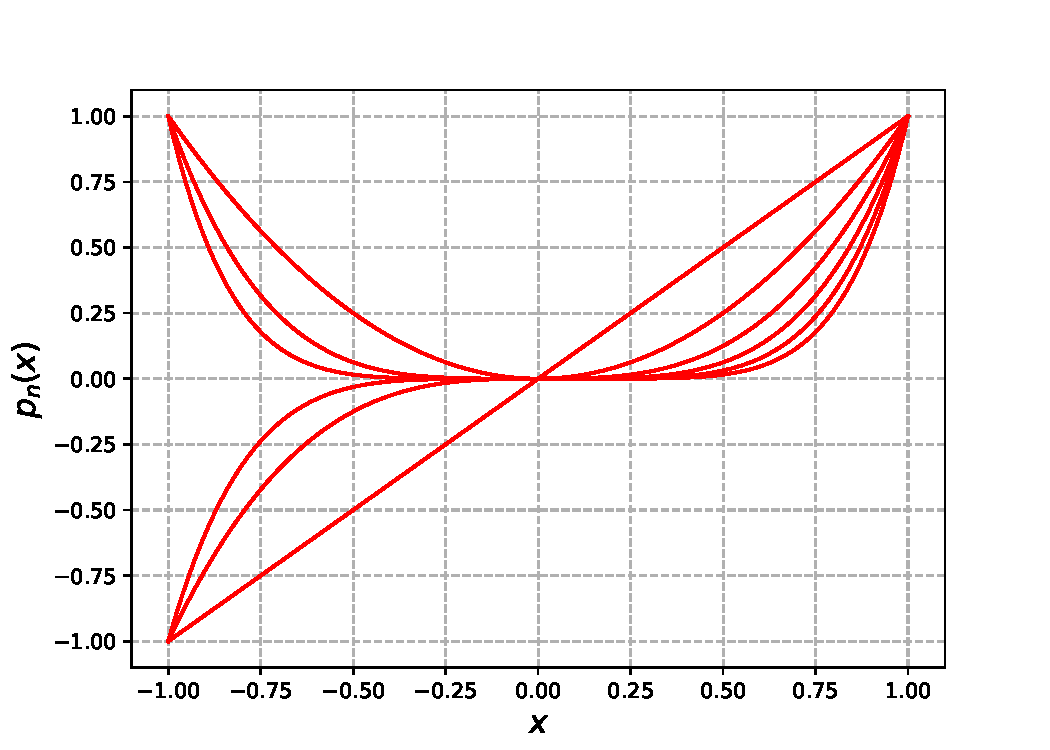
\includegraphics[scale = 0.57]{Figuras/SucesionPolinomios.pdf}
    \caption{Sucesión de polinomios $p_n(x) = x^n, x \in [-1,1]$ para $n = 1, \dots, 6$.}
\end{figure}

Ésta converge en media a $f \equiv 0$. En efecto, 
\begin{align*}
\lim_{n \to + \infty} \int_{-1}^1 |x^n - 0|^2 dx  = \lim_{n \to + \infty }  \int_{-1}^1 x^{2n} \,dx &= \lim_{n \to + \infty} \left. \frac{x^{2n+1}}{2n+1} \right|_{-1}^1 \\
&=  \lim_{n \to + \infty} \frac{2}{2n+1} = 0.
\end{align*}

Sin embargo, no converge puntualmente a $f$ sobre $[-1,1]$, pues 
$$\lim_{n \to + \infty} x^n = \left\{ \begin{array}{cl}
   0 ,& \mbox{si}~ -1 < x < 1 \\
   1  ,&  \mbox{si}~ x = 1 \\
   \mbox{diverge},&  \mbox{si}~ x = -1
\end{array}  \right. .$$

Luego, tampoco uniformemente a $f \equiv 0$ sobre $[-1,1]$.
\end{ejemplo}

\begin{defi}
Considere $f, f_n \in \mathcal{C}[a,b], n \in \mathbb{N}$ y $F_n = \sum\limits_{k=1}^n f_k$. Diremos que la serie $\sum\limits_{n=1}^{\infty} f_n$ \textbf{converge en media} a $f$ si la sucesión de sumas parciales $\{F_n\}_{n\in \mathbb{N}}$ converge en media a $f$. 
\\

\textbf{Notación:} 
$$\sum_{n=1}^{\infty} f_n(t) \sim f(t), \quad t \in [a,b]$$

o 
$$\sum_{n=1}^{\infty} f_n(t) = f(t) ~ [en ~media], \quad t \in [a,b].$$
\end{defi}

\textbf{Observación:}  
\begin{shaded}
$$\sum_{n=1}^{\infty} f_n(t) \sim f(t), \quad t \in [a,b] ~\Leftrightarrow~ \lim_{n \to + \infty} \int_a^b \left[ \sum_{k=1}^n f_k(t) - f(t)\right]^2 \, dt = 0.$$ 
\end{shaded}

\begin{defi}
Una sucesión $\{f_n\}_{n \in \mathbb{N}}$ en $\mathcal{C}[a,b]$ se dice \textbf{sucesión de Cauchy} si dado $\varepsilon > 0$, existe un $N \in \mathbb{N}$ tal que 
$$\forall n,m \geq N ~\Rightarrow~ \norm{f_n-f_m} < \varepsilon.$$
\end{defi}

La definición anterior se puede generalizar a espacios de funciones sin norma, pero con una métrica definida.

Es inmediato verificar que $\{f_n\}_{n \in \mathbb{N}}$ converge a una función $f$ en media, entonces es de Cauchy, pues 
$$\norm{f_n - f_m} \leq \norm{f_n - f} + \norm{f_m - f},$$

y ambos términos en el lado derecho se pueden acotar por un $\varepsilon > 0$ arbitrario para todo $n,m \geq N$. El inverso, sin embargo, es falso, como se puede apreciar en el siguiente ejemplo:

\begin{ejemplo}
Consideremos el conjunto de funciones reales 
 $\mathcal{C}_0[0,1]$, con el producto escalar definido como 
$$\langle f,g\rangle = \int_0^1 f(x) g(x) \,dx.$$

Sea  
\begin{equation*}
    f_n(x) = \left\{ \begin{array}{cl}
       1,  & \mbox{si} ~ 0 \leq x \leq \frac{1}{2}\\
    1 - \left(x - \frac{1}{2} \right)n,     & \mbox{si}  ~ \frac{1}{2} < x < \frac{1}{2} + \frac{1}{n} \\
    0, & \mbox{si} ~ \frac{1}{2} + \frac{1}{n} \leq x \leq 1
    \end{array} \right., n \geq 2.
\end{equation*}

\begin{figure}[H]
    \centering
    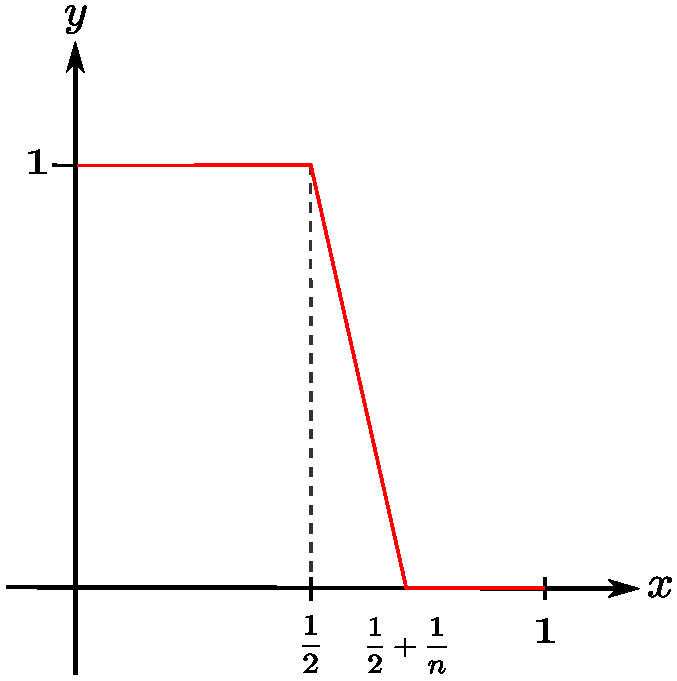
\includegraphics[scale = 0.5]{Figuras/EjemploCauchy.pdf}
    \caption{Ejemplo de sucesión de Cauchy que no converge en media a $C_0[0,1]$.}
\end{figure}

Para $m \geq n$, 
\begin{align*}
    \norm{f_n - f_m}^2 = \int_0^1 |f_n(x) - f_m(x)|^2 \,dx &= \int_0^{\frac{1}{2}} [1-1] \,dx + \int_{\frac{1}{2}}^{\frac{1}{2} + \frac{1}{n}} |f_n(x) - f_m(x)|^2 \,dx + \int_{\frac{1}{2} + \frac{1}{n}}^1 0 \, dx \\
    &=  \int_{\frac{1}{2}}^{\frac{1}{2} + \frac{1}{n}} |f_n(x) - f_m(x)|^2 \,dx.
\end{align*}

Ahora, para todo $x \in \left[\frac{1}{2}, \frac{1}{2}  + \frac{1}{n} \right]$, tenemos

$$|f_n(x) - f_m(x)| \leq |f_n(x)| + |f_m(x)| \leq 1 + 1 = 2. $$

Luego, 
\begin{equation*}
   \norm{f_n - f_m}^2  = \int_{\frac{1}{2}}^{\frac{1}{2} + \frac{1}{n}} |f_n(x) - f_m(x)|^2 \,dx \leq \int_{\frac{1}{2}}^{\frac{1}{2} + \frac{1}{n}} 4 \,dx = \frac{4}{n} ~\Rightarrow~ \norm{f_n - f_m} \leq \frac{2}{\sqrt{n}}.
\end{equation*}

Para $m < n$, es fácil de ver que 
$$\norm{f_n - f_m} \leq \frac{2}{\sqrt{m}}.$$

Así, dado $\varepsilon > 0$, por propiedad arquimediana, existe $N \in \mathbb{N}$ tal que 
$$N > \frac{4}{\varepsilon^2} $$

que verifica 
$$\forall m,n \geq N ~\Rightarrow~   \norm{f_n - f_m} < \varepsilon$$

de modo que es una sucesión de Cauchy. Sin embargo, $\{f_n\}$ converge en media a una función discontinua en $x = \frac{1}{2}$ (pruébelo!), y por lo tanto no converge en $\mathcal{C}_0[0,1]$.
\end{ejemplo}

\begin{defi}
Un espacio normado es llamado \textbf{completo} si toda sucesión de Cauchy es convergente. A un espacio normado completo se le llama \textbf{espacio de Banach}. A un espacio pre-Hilbert que es completo se le llama \textbf{espacio de Hilbert}
\end{defi}

\begin{defi}
El conjunto de funciones $\{\varphi_n(t)\}_{n=0, \pm 1, \pm 2, \dots}$ se dice \textbf{ortogonal} si 
$$\langle \varphi_n , \varphi_m \rangle = 0, \quad \mbox{para} ~ n \neq m.$$

Si además, $\norm{\varphi_n} = 1$ para cada $n \in \mathbb{Z}$, se dice que es un conjunto \textbf{ortonormal}, entonces podemos escribir 
$$\langle \varphi_n , \varphi_m \rangle = \delta_{nm}, \quad \forall n,m.$$
\end{defi}

\begin{ejemplo}
Como ejemplo de funciones ortonormales tenemos las $c_n(t) \in \mathcal{C}_0[-\pi,\pi]$ con $n = 0, \pm 1, \pm 2, \dots$ que se definen como
$$c_n(t) = \frac{1}{\sqrt{2\pi}} e^{i nt}.$$

En efecto, para $n \neq m$, se tiene que
\begin{align*}
    \langle c_n , c_m \rangle = \frac{1}{2\pi} \int_{-\pi}^{\pi} e^{i(n-m)t} \,dt &= \frac{1}{2\pi} \left[ -\frac{i}{n-m} e^{i(n-m) t}\right]_{-\pi}^{\pi} \\
    &= \frac{i}{2\pi(m-n)} [e^{i n\pi} + e^{-i m \pi} - e^{-in \pi} - e^{im \pi}] \\
    &= 0.
\end{align*}

Por otro lado, para $n = m$:
\begin{equation*}
  \langle c_n , c_n \rangle =\frac{1}{2\pi} \int_{-\pi}^{\pi} e^{i(n-n)t} \,dt = \frac{1}{2\pi} \int_{-\pi}^{\pi} 1 \,dt = 1.
\end{equation*}
$$\therefore  \langle c_n , c_m \rangle = \delta_{nm}.$$
\end{ejemplo}

\begin{ejemplo}
Pruebe que el conjunto de funciones 
$$\left\{ \frac{1}{\sqrt{2 \pi}}, \frac{\cos(nt)}{\sqrt{\pi}} ,  \frac{\sin(nt)}{\sqrt{\pi}} \right\}_{n=1}^{\infty}$$

es ortonormal en $\mathcal{C}[-\pi,\pi]$.
\\

\textbf{Solución}: Probemos primero la normalización.
\begin{align*}
    \int_{-\pi}^{\pi} \left( \frac{1}{\sqrt{2\pi}} \right)^2 \,dt &= 1, \\
    \int_{-\pi}^{\pi} \frac{\cos^2(nt)}{\pi} \,dt &=  \frac{1}{\pi} \int_{-\pi}^{\pi} \frac{1}{2} + \frac{1}{2} \cos(2n t) \,dt = 1, \\
    \int_{-\pi}^{\pi} \frac{\sin^2(nt)}{\pi} \,dt &=  \frac{1}{\pi} \int_{-\pi}^{\pi} \frac{1}{2} - \frac{1}{2} \cos(2n t) \,dt = 1.
\end{align*}

Para la ortogonalidad, tengamos en cuenta las siguientes identidades trigonométricas:
\begin{align*}
    \sin \alpha \sin \beta &= \frac{1}{2} [\cos(\alpha - \beta) - \cos(\alpha + \beta)], \\
    \cos \alpha \cos \beta &= \frac{1}{2} [\cos(\alpha - \beta) + \cos(\alpha + \beta)], \\
    \sin \alpha \cos \beta &= \frac{1}{2} [\sin(\alpha + \beta) + \sin(\alpha - \beta)].
\end{align*}

Entonces, 
\begin{align*}
    \int_{-\pi}^{\pi} \frac{1}{\sqrt{2} \pi} \cos(nt) \,dt &=  \left. \frac{1}{\sqrt{2}\pi n} \sin(nt) \right|_{-\pi}^{\pi} = 0, \\
     \int_{-\pi}^{\pi} \frac{1}{\sqrt{2} \pi} \sin(nt) \,dt &=   \left. - \frac{1}{\sqrt{2}\pi n} \cos(nt) \right|_{-\pi}^{\pi} = 0,\\
      \int_{-\pi}^{\pi} \frac{1}{\pi} \cos(n t) \sin(m t)\,dt &=  \frac{1}{2 \pi} \int_{-\pi}^{\pi} \sin(m+n)t + \sin(m-n)t \ dt = 0; \quad n,m \in \mathbb{N}. 
\end{align*}

Para todo $n, m \in \mathbb{N}$, $m \neq n$, se tiene que 
\begin{align*}
    \int_{-\pi}^{\pi} \frac{1}{\pi} \cos(n t) \cos(mt) \,dt &= \frac{1}{2\pi} \int_{-\pi}^{\pi} \cos(n-m)t + \cos(n+m) t\,dt \\
    &= \frac{1}{2\pi} \left[ \frac{1}{n-m} \sin(n-m)t + \frac{1}{n+m} \sin(n+m)t \right]_{-\pi}^{\pi} = 0. \\
     \int_{-\pi}^{\pi} \frac{1}{\pi} \sin(n t) \sin(mt) \,dt &=\frac{1}{2\pi} \int_{-\pi}^{\pi} \cos(n-m)t - \cos(n+m) t\,dt  \\
    &= \frac{1}{2\pi} \left[ \frac{1}{n-m} \sin(n-m)t - \frac{1}{n+m} \sin(n+m)t \right]_{-\pi}^{\pi} = 0.
\end{align*}

Por lo tanto, 
$$\left\{ \frac{1}{\sqrt{2 \pi}}, \frac{\cos(nt)}{\sqrt{\pi}} ,  \frac{\sin(nt)}{\sqrt{\pi}} \right\}_{n=1}^{\infty}$$

es ortonormal en $\mathcal{C}[-\pi,\pi]$.
\end{ejemplo}

\begin{defi}
Sea $S = \{\varphi_n(t)\}_{n=0, \pm 1, \pm 2, \dots}$. Se dice que $S$ es \textbf{linealmente independiente} (l.i.) si todo subconjunto finito de $S$ también lo es.
\end{defi}

\begin{propo} \label{LIortogonal}
Todo conjunto ortogonal en $\mathcal{C}[a,b]$ que no contenga al vector nulo es linealmente independiente.
\end{propo}

\begin{demo}
Sea $S = \{\varphi_n(t)\}_{n=0, \pm 1, \pm 2, \dots}$ ortogonal tal que $\varphi_n \not\equiv 0, \forall n$. Consideremos el subconjunto finito de $S$, $S' = \{\varphi_{i_1}, \dots, \varphi_{i_n}\}$ y además la combinación lineal
$$\alpha_1 \varphi_{i_1} + \alpha_2 \varphi_{i_2} + \cdots + \alpha_n \varphi_{i_n} \equiv 0.$$

Entonces, para un cierto $\varphi_{i_m}$, se tiene que
$$\langle \alpha_1 \varphi_{i_1} + \alpha_2 \varphi_{i_2} + \cdots + \alpha_n \varphi_{i_n},\varphi_{i_m} \rangle = \alpha_m \underbrace{\norm{\varphi_{i_m}}^2}_{\neq 0} = 0.$$

Por lo tanto, 
$$\alpha_m = 0, \quad m = 1, 2, \dots, n$$

probando así que $S'$ es linealmente independiente y en consecuencia $S$ es l.i.
\end{demo}

\section{Proceso de ortonormalización de Gram-Schmidt}

Sea $\{v_n\}_{n = 1,2, \dots}$ un conjunto linealmente independiente de funciones en $\mathcal{C}[a,b]$. Para construir un conjunto ortonormal debemos seguir los siguientes pasos:

\begin{enumerate}
    \item Construimos 
    $$\varphi_1 = \frac{v_1}{\norm{v_1}}$$ 
    
    tal que $\langle \varphi_1 , \varphi_1 \rangle = 1$. 
    
    \item Consideramos
    $$\overline{\varphi}_2 = v_2 - \langle v_2, \varphi_1   \rangle \varphi_1.$$
    
    Entonces, 
    $$\langle \overline{\varphi}_2, \varphi_1 \rangle = \langle v_2, \varphi_1 \rangle - \langle  v_2, \varphi_1  \rangle \langle \varphi_1, \varphi_1 \rangle = \langle v_2, \varphi_1 \rangle -  \langle  v_2, \varphi_1 \rangle  = 0.$$
    
    Normalizando, 
    $$\varphi_2 = \frac{\overline{\varphi}_2}{\norm{\overline{\varphi}_2}}.$$
    
    \item En general para un cierto $n \geq 2$, consideremos 
 $$\overline{\varphi}_n = v_n - \sum_{j=1}^{n-1} \langle  v_n, \varphi_j \rangle \varphi_j.$$
    
Entonces, para $1 \leq  i \leq n-1$, tenemos que
\begin{align*}
    \langle \Bar{\varphi}_n , \varphi_i \rangle &= \langle v_n , \varphi_i \rangle - \sum_{j=1}^{n-1} \langle v_n , \varphi_j \rangle \langle \varphi_j , \varphi_i\rangle \\
    &= \langle v_n, \varphi_i \rangle - \sum_{j=1}^{n-1} \langle v_n , \varphi_j \rangle \delta_{ji} \\
    &= \langle v_n , \varphi_i \rangle -  \langle v_n, \varphi_i \rangle = 0.
\end{align*}
    
Finalmente, normalizando    
$$\varphi_n = \frac{\overline{\varphi}_n}{\norm{\overline{\varphi}_n}}.$$
\end{enumerate}

El conjunto de funciones $\{\varphi_n\}_{n = 1,2, \dots}$ construido de la manera anterior es un conjunto ortonormal.

Geométricamente, el método se encuentra ilustrado en la figura \ref{fig:Gram-Schmidt}, donde se ha considerado las funciones como vectores y solo el proceso de ortogonalización.

\begin{figure}[H]
    \centering
    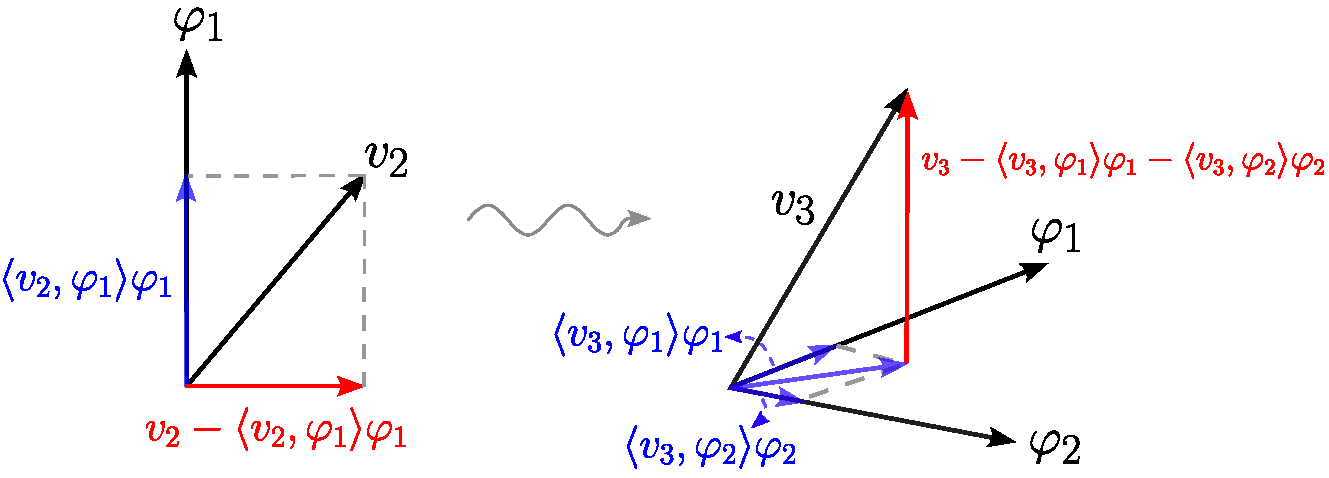
\includegraphics[scale = 0.7]{Figuras/Gram-Schmidt.pdf}
    \caption{Proceso de ortogonalización (sin la normalización) de Gram-Schmidt para tres funciones $\{v_1,v_2,v_3\}$.}
    \label{fig:Gram-Schmidt}
\end{figure}

\newpage
\section{Coeficientes de Fourier}

Ahora, definiremos un espacio de funciones más general que $\mathcal{C}[a,b]$, las funciones cuadrado integrables. \footnote{La condición de cuadrado integrable es usada, por ejemplo, en Mecánica Cuántica, pues constituye la base para que las funciones de onda describan el comportamiento de los sistemas físicos, consecuencia de la interpretación de Copenhague (probabilística) de la mecánica cuántica.}

\begin{defi}
    Definimos $\mathcal{L}^2[a,b]$ como el espacio de funciones $f:[a,b] \rightarrow \mathbb{C}$, tales que 
    $$\int_a^b |f(t)|^2 \,dt < \infty.$$
\end{defi}

\begin{teorema}
El espacio $\mathcal{L}^2[a,b]$ es un espacio vectorial con producto interno 
$$\langle f,g \rangle = \int_a^b f(t) g^* (t) \,dt$$

y norma
$$\norm{f} = \left( \int_a^b |f(t)|^2 \,dt \right)^{1/2}.$$
\end{teorema}

La demostración requiere verificar las propiedades del producto interno (escalar) dadas por \ref{ProductoEscalar}, la cual está fuera de los alcances de los contenidos de este apunte. \footnote{Para más información puede consultar bibliografía relacionada a la integral de Lebesgue.} 

\textbf{Observación:} Las funciones seccionalmente continuas son funciones cuadrado integrables.
\\

Sea $\{\varphi_{\nu}(t)\}_{\nu \in \mathbb{N}}$ un conjunto ortonormal de funciones tales que $\varphi_{\nu} \in \mathcal{C}[a,b]$ para todo $\nu \in \mathbb{N}$. Sea $f(t)$ una función cuadrado integrable en $[a,b]$. Deseamos aproximar $f(t)$ por una suma finita 
$$S_n(t) = \sum_{\nu = 1}^n C_{\nu} \varphi_{\nu}(t),$$

de manera que $\norm{f - S_n}$ sea mínimo. Es decir, el objetivo es encontrar los coeficientes $C_{\nu}$ de modo que el \textbf{error cuadrático medio}
$$M_n(f) = \norm{f-S_n}^2 = \int_a^b \left| f(t) - \sum_{\nu = 1}^n C_{\nu} \varphi_{\nu}(t) \right|^2 \,dt,$$

sea mínimo. Evaluemos el error cuadrático medio
\begin{align}
    M_n(f) &= \int_a^b \left( f(t) - \sum_{\nu = 1}^n C_{\nu} \varphi_{\nu}(t)  \right) \left( f(t) - \sum_{\nu = 1}^n C_{\nu} \varphi_{\nu}(t) \right)^* \,dt \nonumber \\
    &= \int_a^b |f(t)|^2 \, dt  + \sum_{\nu = 1}^n |C_{\nu}|^2 \int_a^b |\varphi_{\nu}(t)|^2 \,dt - \sum_{\nu = 1}^n C_{\nu}^* \int_a^b f(t) \varphi_{\nu}^*(t) \,dt \nonumber \\
    & \quad - \sum_{\nu = 1}^n C_{\nu} \int_a^b f^*(t) \varphi_{\nu}(t) \,dt  \nonumber \\
    &= \norm{f}^2 + \sum_{\nu = 1}^n |C_{\nu}|^2 - \sum_{\nu = 1}^n C_{\nu}^* \langle f, \varphi_{\nu} \rangle - \sum_{\nu = 1}^n C_{\nu} \langle f, \varphi_{\nu} \rangle^* + \sum_{\nu = 1}^n |\langle f, \varphi_{\nu} \rangle|^2 - \sum_{\nu = 1}^n |\langle f, \varphi_{\nu} \rangle|^2\nonumber  \\
    &= \norm{f}^2  - \sum_{\nu = 1}^n |\langle f, \varphi_{\nu} \rangle|^2 + \sum_{\nu = 1}^n |C_{\nu} - \langle f , \varphi_{\nu} \rangle|^2 \geq 0, \label{ErrorMedio}
\end{align}

ya que la norma es mayor o igual a cero siempre. Claramente el mínimo se obtiene cuando $C_{\nu} = \langle f, \varphi_{\nu} \rangle$. 

De lo anterior se desprende: 
\begin{shaded}
 \begin{equation}
 \sum_{\nu = 1}^n |C_{\nu}|^2 = \sum_{\nu = 1}^n |\langle f , \varphi_{\nu} \rangle|^2 \leq \norm{f}^2  \qquad \mbox{\textbf{Desigualdad de Bessel}} \label{D.Bessel}.
\end{equation}
 
\end{shaded}

Como el número a la derecha de la desigualdad es independiente de $n$, la suma está acotada superiormente. Siendo todos sus términos no negativos, tenemos que
$$\sum_{\nu = 1}^{\infty} |C_{\nu}|^2 < \infty ~\Rightarrow~ \lim_{\nu \to + \infty} |C_{\nu}|^2 = 0 ~\Rightarrow ~ \lim_{\nu \to + \infty} \langle f , \varphi_{\nu} \rangle = 0.$$

Luego,
\begin{equation*}
 \sum_{\nu = 1}^{\infty} |C_{\nu}|^2 = \sum_{\nu = 1}^{\infty} |\langle f , \varphi_{\nu} \rangle|^2 \leq \norm{f}^2    .
\end{equation*}

\begin{defi}
Los coeficientes $\langle f , \varphi_{\nu}\rangle$ son llamados los \textbf{coeficientes de Fourier} de $f$  respecto al sistema ortonormal $\{\varphi_{\nu}\}_{\nu = 1,2, \dots}$. La serie $\sum\limits_{\nu = 1}^{\infty} C_{\nu} \varphi_{\nu}(t)$ se llama \textbf{serie generalizada de Fourier} de $f$ relativa al sistema ortonormal $\{\varphi_{\nu}\}_{\nu = 1,2, \dots}$.

\end{defi}

\begin{defi}
Si un conjunto de funciones $\{\varphi_{\nu}\}$ en cierto espacio permite aproximar en la norma (en media), con sus combinaciones lineales, cualquier función $f$ del espacio tan bien como se quiera, es decir,
$$\left\Vert f - \sum_{\nu} C_{\nu} \varphi_{\nu} \right\Vert< \varepsilon, \qquad \mbox{para $\varepsilon$ arbitrario},$$

se dice que es un \textbf{conjunto completo} respecto a este espacio.
\end{defi}

Sean $C_{\nu} = \langle f , \varphi_{\nu} \rangle$ los coeficientes de Fourier de $f$ respecto del conjunto ortonormal  $\{\varphi_{\nu}\}$, entonces la completitud de este conjunto se puede expresar por 
$$\lim_{n \to + \infty} \left\Vert f - \sum_{\nu =1}^{n} C_{\nu} \varphi_{\nu} \right\Vert = 0,$$

es decir, 
$$f \sim \sum_{\nu = 1}^{\infty} C_{\nu} \varphi_{\nu}.$$

Lo anterior NO implica que $f(t) = \sum\limits_{\nu = 1}^{\infty} C_{\nu} \varphi_{\nu}(t)$ en algún otro sentido (convergencia puntual o uniforme). Si
$$f \sim \sum_{\nu = 1}^{\infty} C_{\nu} \varphi_{\nu},$$

entonces de la relación \eqref{ErrorMedio}, tenemos 
\begin{equation*}
    \lim_{n \to + \infty} \left\Vert f - \sum_{\nu = 1}^n  C_{\nu} \varphi_{\nu} \right\Vert^2 = \lim_{n \to + \infty} \left\{ \Vert f \Vert^2 - \sum_{\nu = 1}^{n} |C_n|^2 \right\} = \norm{f}^2  - \sum_{\nu = 1}^{\infty} |C_n|^2 = 0.
\end{equation*}

Lo que implica que
\begin{shaded}
 \begin{equation}
    \norm{f}^2  = \sum_{\nu =1 }^{\infty} |C_{\nu}|^2 \qquad \mbox{\textbf{Igualdad de Parseval}}
\end{equation}   
\end{shaded}

\textbf{Observación:} El conjunto ortogonal completo $\{\varphi_{\nu}\}$ se le conoce también como \textbf{base ortogonal} del espacio de funciones en cuestión.

\begin{ejemplo}
El conjunto $\left\{ \frac{1}{\sqrt{2 \pi}} e^{i n t} \right\}_{n \in \mathbb{Z}}$ es ortonormal completo respecto a $[-\pi,\pi]$.
$$f(t) \sim \sum_{n = - \infty}^{\infty} C_n \frac{e^{int}}{\sqrt{2\pi}} ~\Rightarrow~ \int_{-\pi}^{\pi} |f|^2 \,dt = \sum_{n=- \infty}^{\infty} |C_n|^2 = \norm{f}^2 .$$
\end{ejemplo}


\begin{teorema}{}{} 
Si el conjunto ortonormal $\{\phi_{\nu}\}$ es completo respecto a $\mathcal{C}[a,b]$, entonces en $\mathcal{C}[a,b]$ la única función ortonormal a todo $\varphi_{\nu}$ es $f(t) \equiv 0$.
\end{teorema}

\begin{demo}
Sea $f$ una función ortonormal a todo $\varphi_{\nu}$, si $f(t_0) \neq 0$ para algún $t_0 \in [a,b]$, la función también es no nula en una vecindad en torno a $t_0$ (por continuidad), por lo tanto 
$$\int_a^b |f(t)|^2 \,dt = \norm{f}^2  > 0,$$

pero usando la igualdad de Parseval, tenemos para la norma de $f$ que
$$\norm{f}^2  = \sum_{\nu} |C_{\nu}|^2 = \sum_{\nu} |\langle f ,\varphi_{\nu} \rangle|^2 > 0,$$

es decir, $f$ no es ortogonal a todos los $\varphi_{\nu}$, lo cual es una contradicción. Luego, $f$ debe ser idénticamente nula.
\end{demo}

\begin{teorema}
Sea $\{S_n(t) \in \mathcal{C}_0[a,b]\}$; si existe $F(t)$ tal que la sucesión $S_n(t) = \sum\limits_{\nu = 1}^n C_{\nu} \varphi_{\nu}(t)$ converge uniformemente a $F(t)$, entonces $F(t)$ es continua, es decir, $F(t) \in \mathcal{C}_0[a,b]$.
\end{teorema}

\begin{demo}
Por convergencia uniforme, dado $\varepsilon > 0$, $\exists N \in \mathbb{N}$ tal que
$$n \geq N \wedge \forall t \in [a,b] ~\Rightarrow~ |S_n(t) - F(t)| < \frac{\varepsilon}{3}.$$

Además, por la continuidad de $S_n$ para todo $t_0 \in [a,b]$, existe $\delta(\varepsilon, N, t_0)$ tal que
$$\forall t \in [a,b]: ~ 0 < |t-t_0| < \delta ~\Rightarrow~ |S_N(t) - S_N(t_0)| < \frac{\varepsilon}{3}.$$

Por lo tanto, 
\begin{align*}
 \forall t \in [a,b]: ~ 0 < |t-t_0| < \delta &\Rightarrow |F(t) - F(t_0)|  \\
 &= |F(t) - S_n(t) + S_n(t) - S_n(t_0) + S_n(t_0) - f(t_0)| \\
 &\leq |F(t) - S_n(t)| + |S_n(t) - S_n(t_0)| + |S_n(t_0) - F(t_0)| \\
 &\leq \frac{\varepsilon}{3} + \frac{\varepsilon}{3} + \frac{\varepsilon}{3} = \varepsilon .
\end{align*}
\end{demo}

Este teorema nos asegura que una función discontinua no puede ser aproximada uniformemente por una familia de funciones continuas (por ejemplo, las funciones sinusoidales).

\begin{teorema}
Si dos funciones $f,g \in \mathcal{C}[a,b]$ tienen igual expansión en base completa (en el sentido de aproximación en la norma), entonces $f(t) = g(t)$.
\end{teorema}

\begin{demo}
Sea
$$S(t) = \sum_{\nu = 1}^{\infty} \langle f, \varphi_{\nu}\rangle \varphi_{\nu}(t)$$

la aproximación en la norma para $f$ y $g$. Luego, 
$$\Vert f-S \Vert = \Vert g-S \Vert = 0.$$

Así, 
\begin{equation*}
    \Vert f-g \Vert = \Vert f-S+S-g \Vert \leq \Vert f-S \Vert + \Vert S-g \Vert = 0 +0 = 0 ~\Rightarrow~ f = g.
\end{equation*}

\end{demo}

\section{Convergencia según Cesàro*}

Si consideramos la serie
$$\frac{1}{1-x} = \sum_{n=1}^{\infty} x^{n-1} = 1 + x + x^2 + x^3 + \cdots$$

ella converge para $|x|< 1$. A pesar de lo anterior evaluemos la función y su expansión en serie en $x = -1$:
$$\left. \frac{1}{1-x} \right|_{x= -1} \overset{?}{=} \frac{1}{2} = 1 - 1 + 1 -1 +1 -1 + \cdots$$

¿Será posible sumar la serie de modo que ésta sí converja al valor de la función en ese punto?

\begin{defi}
Sea $s_n$ la suma parcial $n$-ésima de la serie $\sum\limits_{n=1}^{\infty} a_n$ y sea $\{\sigma_n\}_{n\in \mathbb{N}}$ la sucesión de las medias aritméticas definidas por
$$\sigma_n = \frac{s_1 + \cdots + s_n}{n}, \quad n = 1, 2, \dots$$

La serie $\sum\limits_{n=1}^{\infty} a_n$ es \textbf{sumable de Cesàro} si $\{\sigma_n\}_{n\in \mathbb{N}}$ converge. Si $\lim\limits_{n \to + \infty} \sigma_n = S^*$, entonces $S^*$ se llama \textbf{suma de Cesàro} de $\sum\limits_{n=1}^{\infty} a_n$ y se escribe 
$$ \sum_{n=1}^{\infty} ^*   a_n = S^*.$$
\end{defi}

\begin{ejemplo}
Sea $a_n = x^{n-1}$ con $x \neq 1$. Entonces
$$s_n = \frac{1}{1-x} - \frac{x^n}{1-x} \qquad \mbox{(Demuéstrelo!!)}$$

y
\begin{align*}
 \sigma_n = \frac{1}{n} \sum_{k=1}^n \left\{\frac{1}{1-x} - \frac{x^k}{1-x} \right\} &= \frac{1}{1-x} - \frac{1}{n(1-x)} \sum_{k =1}^{n} x^k   \\
 &=\frac{1}{1-x} -  \frac{1}{n} \frac{x(1-x^n)}{(1-x)^2}.
\end{align*}

Por consiguiente, 
$$\sum_{n=1}^{\infty}^* x^{n-1} = \lim_{n \to +\infty} \left\{ \frac{1}{1-x} -  \frac{1}{n} \frac{x(1-x^n)}{(1-x)^2}\right\} = \frac{1}{1-x}; \quad |x| \leq 1, x \neq 1. $$

En particular,
$$\sum_{n=1}^{\infty}^* (-1)^{n-1} = \frac{1}{2}.$$

\end{ejemplo}

Note que la idea de la definición de sumabilidad de Cesàro es encontrar una forma de dar significado a series que en otro caso serían divergentes.
\\

\textbf{Observación}: La convergencia ordinaria necesita que el $\lim\limits_{n \to + \infty} \sum\limits_{k = 1}^n a_{k}$ exista. 

\hspace{2.45cm} La convergencia según Cesàro necesita que el $\lim\limits_{n \to + \infty} \frac{1}{n} \sum\limits_{k = 1}^n  \sum\limits_{l = 1}^{k} a_{l}$ exista.

\begin{teorema}
Si una serie es convergente con suma $S$, entonces es sumable de Cesàro con suma $S^* = S$.
\end{teorema}

Problemas similares a la serie discreta anterior ofrece calcular la integral, desde cero hasta infinito, de una función oscilante, que no decrece, del tipo $\int_0^{\infty} \sin(\omega x) \,dx$.

En el espíritu del caso discreto, proponemos la siguiente definición.

\begin{defi}
Definimos una \textbf{integral de Cesàro} de la siguiente manera:
\begin{equation}
    ^* \int_0^{\infty} f(t) \,dt = \lim_{y \to \infty } \frac{1}{y} \left\{ \int_0^y \int_0^x f(t) \,dt dx \right\}. \label{IntegralCesaro1}
\end{equation}

\end{defi}


Podemos encontrar una expresión alternativa para la integral de Cesàro integrando por partes la ecuación \eqref{IntegralCesaro1}:
\begin{align*}
    ^* \int_0^{\infty} f(t) \,dt &= \lim_{y \to \infty } \frac{1}{y} \left\{ \int_0^y \int_0^x f(t) \,dt dx \right\} \\
    &= \lim_{y \to \infty } \frac{1}{y} \left\{\left. x \int_0^x f(t)\,dt \right|_0^y - \int_0^y x f(x) \,dx \right\} \\
    &= \lim_{y \to \infty } \frac{1}{y} \left\{ y \int_0^y f(t) \,dt - \int_0^y xf(x) \,dx \right\}
\end{align*}
\begin{equation}
    \Rightarrow ~  \boxed{^* \int_0^{\infty} f(t) \,dt = \lim_{y \to \infty} \int_0^y \left( 1 - \frac{x}{y} \right) f(x) \,dx} \label{IntegralCesaro2}
 \end{equation}
 
 \begin{ejemplo}
Evalúe la integral de Cesàro de la función $f(x) = \sin(\omega x)$ con $\omega \neq 0$.
\\

\textbf{Solución:} Usando la ecuación \eqref{IntegralCesaro1}, obtenemos que
\begin{align*}
      ^* \int_0^{\infty} \sin(\omega t) \,dt &= \lim_{y \to \infty } \frac{1}{y} \left\{ \int_0^y \int_0^x \sin(\omega t) \,dt dx \right\} \\
      &= \lim_{y \to \infty } \frac{1}{y} \int_0^y \left[ \frac{1 - \cos(\omega x)}{\omega}\right] \, dx \\
      &= \lim_{y \to \infty} \left[ \frac{1}{\omega} - \frac{1}{\omega^2} \frac{\sin(\omega y)}{y}\right]
\end{align*}
\begin{equation}
    \Rightarrow ~  \boxed{^* \int_0^{\infty} \sin(\omega t) \,dt = \frac{1}{\omega}} \label{CesaroSeno}
 \end{equation}

 \end{ejemplo}
 
  \begin{ejemplo}
Evalúe la integral de Cesàro de la función $f(x) = \cos(\omega x)$ con $\omega \neq 0$.
\\

\textbf{Solución:} Usando la ecuación \eqref{IntegralCesaro1}, obtenemos que
\begin{align*}
      ^* \int_0^{\infty} \cos(\omega t) \,dt &= \lim_{y \to \infty } \frac{1}{y} \left\{ \int_0^y \int_0^x \cos(\omega t) \,dt dx \right\} \\
      &= \lim_{y \to \infty } \frac{1}{y} \int_0^y \frac{\sin(\omega x)}{\omega} \, dx \\
      &= \lim_{y \to \infty} \left[ \frac{1}{\omega^2 y} - \frac{\cos(\omega y)}{\omega^2 y} \right]
\end{align*}
\begin{equation}
    \Rightarrow ~  \boxed{^* \int_0^{\infty} \cos(\omega t) \,dt = 0 } \label{CesaroCoseno}
 \end{equation}

 \end{ejemplo}

\nocite{*} %Referencia todo, incluso lo que no está citado.
\printbibliography[title={Referencias}]

\end{document}
